We begin by defining a formal model for describing surveillance strategy synthesis problems, in the form of a two-player game between an agent and a target, in which the agent has only partial information about the target's location. We first present the game structure with all its components, and then explain each component. We broadly categorize the structure's components into \emph{sensing} and \emph{transitions}. 

Since the focus of this paper is on high-level decision making, we abstract the sensing capabilities into a generic model. This ensures that most sensor models in practice can be captured in the presented framework. 

\subsection{Notation}\label{sec:notation}
We first introduce some notation necessary for the formal definitions in the remainder of the section. For a finite set $B$, we denote with $|B|$ the number of elements in B. Given a set $B$, we denote with $\mathcal{P}(B) = \{B' \mid B'\subseteq B\}$ the powerset (set of all subsets) of $B$. Note that $|\mathcal{P}(B)|=2^{|B|}$. 

We use $\mathbb N$ to denote the set of natural numbers, and $\mathbb N_{>0}$ to denote the set of positive natural numbers.


\subsection{Surveillance Game Structures}\label{sec:surveillance-games}
Given an environment with a discrete finite set of possible locations $L$, we define a \emph{surveillance game structure} to be  a tuple $G  = (\states,s^\init,\trans,\sense,\mathcal{M},\obs)$, where:
\begin{itemize}
\item $\states = L \times L$ is the \emph{set of states}, where for each state $(l_a,l_t) \in S$ we interpret $l_a \in L$ as the location of the agent, and $l_t \in L$ as the location of the target;
\item $s^\init = (l_a^\init,l_t^\init) \in S$ is the initial state;
\item $\trans \subseteq \states \times \states$ is the \emph{transition relation} describing the possible moves of the agent and the target; 
\item $\sense : \states \to \mathbb{B} \times (\mathcal{P}(L)\cup \{\bot\})$ is a \emph{sensing function} that maps a state $(l_a,l_t)$ to a pair $(b,U)$, where $b$ is \emph{true} iff \emph{location $l_t$ can be sensed by the agent from $l_a$}, and when $b$ is \emph{true}, then $U \in \mathcal{P}(L)$ is the set of possible locations of the target returned by the agent's sensor and $l_t \in U$. Formally, if $\sense(l_a,l_t) = (b,U)$ we require that:
\begin{enumerate}
    \item if $b = \true$, then $l_t \in U$, and
    \item if $b = \false$, then $U = \bot$.
\end{enumerate}
\item $\mathcal{M} = \{\Lambda_1,\dots,\Lambda_m\}$ is a possibly empty set of \emph{static sensors}, where $\Lambda_i \in \mathcal{P}(L) \setminus \{\emptyset\}$ is the non-empty set of locations over which the $i$-th static sensor operates.
\item $\obs : \states \to \mathcal{P}(L)$ is an \emph{observation function} that maps each state $(l_a,l_t)$ to a set of locations in $L$, corresponding to the information that the agent receives from all sensors regarding the possible locations of the target, when the agent is in location $l_a$ and the target is in location $l_t$.
\end{itemize}

\begin{figure}
	\centering
\subfloat[Sensor output when target is in sensor range \label{fig:simple-sensing-vis-perf}]{
\input{Surveillance/figs/7x7_perfect_sensing_example.tex}}\hspace{0.06 in}
\subfloat[Sensor output when target is not visible \label{fig:simple-sensing-invis}]{
\input{Surveillance/figs/7x7.tex}
} \hspace{0.05 in}
\subfloat[Sensor output for an imperfect sensor \label{fig:simple-sensing-vis-imperf}]{
\input{Surveillance/figs/7x7_imperfect_sensor_example.tex}}
\hfill
\caption[A simple surveillance game on a grid arena]{A simple surveillance game on a grid arena. The agent is shown in blue, the target in orange, and obstacles in red. Grey locations depict the current observation the agent receives as output from the sensors.}
\label{fig:simple-sensing}
\end{figure}

\subsubsection*{\textbf{Sensing and observation}} In the following, we define the \emph{sensing} and \emph{observation} components of the surveillance game structure. We first present the observation function $\obs$ informally. Simply, $\obs$ maps the joint state of the agent and target to a set of possible locations of the target. The function $\obs$ incorporates the information from all available sensor modalities and static sensors available to the agent. More precisely, $\obs$ combines the information the agent receives from its own sensors, here given by the $\sense$ function, and the information received by the static sensors $\mathcal M$. 

We begin by presenting the function $\sense$ in detail. As stated above, the function $\sense$ maps a state $(l_a,l_t)$ to a pair $(b,U) \in \mathbb{B} \times (\mathcal{P}(L) \cup \{\bot\})$ such that $b$ indicates whether location $l_t$ can be sensed by the agent when it is located at $l_a$.

If we assume \emph{perfect sensing}, whenever $b$ is $\true$, the set $U$ will consist of a single element, which is the \emph{actual location} $l_t$ of the target. If the sensor has \emph{uncertainty}, then whenever $b$ is $\true$, then the set $U$ contains \emph{all possible locations} of the target given the sensor output. We assume that the actual location $l_t$ of the target is always among the ones in the set $U$. 
For example, $U$ can be the support of a probability distribution over possible locations from a probabilistic sensor model. 

\bigskip
\begin{eg}\label{ex:simple-surveillance-game-perfect-sensing}
Figure~\ref{fig:simple-sensing} shows an example of a surveillance game on a grid.  The set of possible locations $L$ for the agent and the target consists of the cells of the  grid. We assume that the agent is equipped with a line-of-sight sensor, that is, location $l_t$ is visible from a location $l_a$ if there is no obstacle on the straight line between them.

Figure~\ref{fig:simple-sensing-vis-perf} depicts the case where the agent has perfect sensing. In this case, for state $(4,19)$ the sensor function returns $\sense(4,19) = (\true,\{19\})$, where the set returned by the sensor contains only the true location of the target. 

If the agent is at location $l_a = 4$, and the target is at location $l_t = 18$, the agent, equipped with line-of-sight sensor, cannot sense the target.
Thus, $\sense(4,18) = (\false,\bot)$.
\qed
\end{eg}

\bigskip
\begin{eg}\label{ex:simple-surveillance-game-imperfect-sensing}
Consider the game in Figure~\ref{fig:simple-sensing}, and let us now examine the case of imperfect sensing. Suppose that we have a line-of-sight sensor, which this time has limited precision. More precisely, its worst-case uncertainty is parametrized by $\lambda$ where $\lambda$ is the largest number of possible locations that the target can be in, given a sensor reading. For example, if $\lambda = 6$, a possible sensor reading for state $(4,6)$ returns $\sense(4,6) = (\true, \{1,2,3,6,7,8\})$, as depicted in Figure~\ref{fig:simple-sensing-vis-imperf}. 
\qed
\end{eg}

\bigskip

Before we can define the observation function $\obs$, we need to provide the semantics of the static sensors $\mathcal{M} = \{\Lambda_1,\dots,\Lambda_m\}$. In the definition of $\mathcal M$, we identify a \emph{static sensor} with a \emph{non-empty set of locations $\Lambda \subseteq L$ over which it operates}. Simply, such a static sensor lets the agent know if a target has entered a location in $\Lambda$. The static sensor cannot distinguish which \emph{specific} location the target is in, only whether it is currently in its operating region or not. 
We assume that the static sensors do not suffer from false positives or negatives (studying these is an avenue for future work). 

Each location can be in the operating region of multiple static sensors. Given a location $l_t \in L$, we define $J(l_t)$ to be the set of all indices of static sensors such that $l_t$ belongs to the corresponding set of locations, i.e, 
$J(l_t) := \{j \in \{1,\ldots,m\}\mid l_t\in \Lambda_j\}.$
We refer to $J(l_t)$ as the set of \emph{triggered static sensors}  when the target is at location $l_t$. 
Thus, by definition, if static sensors have been triggered we have that the target is in the intersection of the areas of operation of the triggered sensors, i.e., $$ J(l_t) \neq \emptyset \implies l_t \in \left(\bigcap_{j\in J(l_t)}\Lambda_j\right) \setminus \left(\bigcup_{j\not\in J(l_t)}\Lambda_j\right).$$ Also, when no static sensor is triggered, the target is outside of the union of the operating regions of all static sensors i.e, $$J(l_t) = \emptyset \implies l_t \notin \bigcup_{i=1}^m \Lambda_i.$$

Based on these observations, we define a function $\sense_{static}: L \to \mathcal{P}(L)$ that maps a location of the target to the \emph{joint output of the static sensors $\mathcal M$} as follows:
\begin{itemize}
    \item if $J(l_t) \neq \emptyset$, then 
\[\sense_{static}(l_t) := \left(\bigcap_{j\in J(l_t)}\Lambda_j\right) \setminus \left(\bigcup_{j\not\in J(l_t)}\Lambda_j\right);\]
    
    \item if $J(l_t) = \emptyset$, then
\[\sense_{static}(l_t) := L \setminus \left(\bigcup_{i=1}^m \Lambda_i\right).\]
\end{itemize}
%\[
%    \sense_{static}(l_t) := \begin{cases}
%         \left(\bigcap_{j\in J(l_t)}\Lambda_j\right) \setminus \left(\bigcup_{j\not\in J(l_t)}\Lambda_j\right) & \text{if } J(l_t) \neq \emptyset \\
%         L \setminus \left(\bigcup_{i=1}^m \Lambda_i\right) & \text{if } J(l_t) = \emptyset.
%        \end{cases}
%\]


\begin{figure}
\centering
\subfloat[Sensor output with no static sensor triggered \label{fig:simple-sensing-static}]{
\input{Surveillance/figs/7x7_static_sensor.tex}
} \hspace{0.45 in}
\subfloat[Sensor output when static sensor is triggered \label{fig:simple-sensing-static-triggered}]{
\input{Surveillance/figs/7x7_static_sensor_triggered.tex}}
\hfill
\caption[A surveillance game example with static sensors.]{A simple surveillance game on a grid arena. The agent is shown in blue, the target in orange, and obstacles in red. Yellow locations correspond to the area on which the static sensor operates. Grey locations depict the current observation the agent receives as output from all the sensors.}
\label{fig:simple-sensing-static-sensors}
\end{figure}

\bigskip
\begin{eg}\label{ex:simple-surveillance-game-static-sensing}
Figure~\ref{fig:simple-sensing-static} shows an example game structure with a static sensor operating over the yellow locations in the grid environment. Formally, we have $\mathcal{M} = \{\Lambda_1\}$ where $\Lambda_1 = \{10,15,20\}$. 
For the configuration depicted in Figure~\ref{fig:simple-sensing-static}, the output of the static sensor is $\sense_{static}(16) = L \setminus \{10,15,20\}$, corresponding to the information that the target is not in any of the locations on which it operates. 

If the target is in location $15$, as shown in Figure~\ref{fig:simple-sensing-static-triggered}, the output of the static sensor is $\sense_{static}(15) = \{10,15,20\}$, corresponding to the locations on which $\Lambda_1$ operates. 
\qed
\end{eg}

We are now ready to present the formal definition of the \emph{observation function $\obs$}, which merges the output of the agent's sensor with the output of the static sensors, to provide the joint observation that the agent makes at a given state $(l_a,l_t)$. Formally, the function $\obs$ is fully defined by the functions $\sense$ and $\sense_{static}$ presented above.

We first define a \emph{visibility function} 
$$\vis(l_a) := \{l \in L \mid \exists U \subseteq L: \sense(l_a,l) = (\true,U)\},$$ which maps the agent's location $l_a$ to the set of all locations in the game structure that are visible from location $l_a$.

Finally, we define $\obs: S \to \mathcal{P}(L)$ such that:
\begin{itemize}
    \item if $\sense(l_a,l_t) =  (\true,U)$, then
 $$\obs(l_a,l_t) :=  (U \cap \vis(l_a) )\cap \sense_{static} (l_t)\text{, and}$$
    \item if $\sense(l_a,l_t) =  (\false,\bot)$, then
$$\obs(l_a,l_t) := \sense_{static}(l_t) \setminus \vis(l_a).$$
\end{itemize}
Intuitively, if the target is in some location visible for the agent, then the set of possible locations of the target is the intersection of the sets of possible visible locations returned by the agent's sensor and the static sensors.
If, on the other hand, the target is in a location that is not visible, then the set of possible locations of the target consists of all locations returned by the static sensors, minus those visible from  $l_a$.


Note that for every state $(l_a,l_t)$ we have that $l_t \in \obs(l_a,l_t)$.

We denote with $\range(\obs)$ the range of the function $\obs$, i.e., $\range(\obs) = \{O \subseteq L \mid \exists (l_a,l_t) \in S : \obs(l_a,l_t) = O\}$.

\bigskip
\begin{eg}
The gray regions in Figure~\ref{fig:simple-sensing} and  Figure~\ref{fig:simple-sensing-static} depict the output of function $\obs$ in the different cases. 

For instance, in Figure~\ref{fig:simple-sensing-invis} there are no static sensors, and thus, function $\obs$ returns the set of possible locations according to function $\sense$. Thus, the set $\obs(4,18) = \{10,15,16,17,18,20,21,22,23\}$ consists of all locations that are not visible from the agent's location $4$, and the set $\obs(4,6) = \{1,2,3,4,6,7\}$ consists of all locations in the uncertainty set $U$, where $\sense(4,6) = (\true,U)$.

The examples in Figure~\ref{fig:simple-sensing-static}, on the other hand, contain the static sensor $\Lambda_1$, defined in Example~\ref{ex:simple-surveillance-game-static-sensing}. In Figure~\ref{fig:simple-sensing-static} the static sensor is not triggered, and thus $\obs$ returns the set of locations that are not visible from the agent's location and do not belong to the yellow area. In Figure~\ref{fig:simple-sensing-static-triggered}, on the other hand, the static sensor is triggered and the output of $\obs(4,15)$ is $\{10,15,20\}$ which corresponds to the set of locations $\Lambda_1$.
\qed
\end{eg}



\begin{figure}
	\centering
\subfloat[Surveillance arena \label{simple-grid}]{

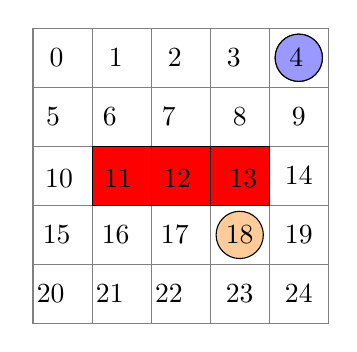
\begin{tikzpicture}[scale=1.5]
\draw[step=0.5cm,color=gray] (-1.5,-1.5) grid (1,1);
\filldraw[fill=blue,draw=black] (+0.75,+0.75) circle (0.2cm);
\filldraw[fill=red,draw=black] (0,0) rectangle (-0.5,-0.5);
\filldraw[fill=red,draw=black] (-0.5,0) rectangle (-1,-0.5);
\filldraw[fill=red,draw=black] (0,0) rectangle (0.5,-0.5);
\filldraw[fill=blue!40!white,draw=black] (+0.75,+0.75) circle (0.2cm);
\filldraw[fill=orange!40!white,draw=black] (0.25,-0.75) circle (0.2cm);
\node at (-1.30,+0.75) {{0}};
\node at (-0.80,+0.75) {{1}};
\node at (-0.30,+0.75) {{2}};
\node at (0.20,+0.75) {{3}};
\node at (0.73,+0.75) {{4}};
\node at (-1.33,+0.25) {{5}};
\node at (-0.85,+0.25) {{6}};
\node at (-0.35,+0.25) {{7}};
\node at (0.25,+0.25) {{8}};
\node at (0.75,+0.25) {{9}};
\node at (-1.28,-0.27) {{10}};
\node at (-0.78,-0.27) {{11}};
\node at (-0.28,-0.27) {{12}};
\node at (0.28,-0.27) {{13}};
\node at (0.75,-0.25) {{14}};
\node at (-1.3,-0.75) {{15}};
\node at (-0.8,-0.75) {{16}};
\node at (-0.3,-0.75) {{17}};
\node at (0.25,-0.75) {{18}};
\node at (0.75,-0.75) {{19}};
\node at (-1.35,-1.25) {{20}};
\node at (-0.85,-1.25) {{21}};
\node at (-0.35,-1.25) {{22}};
\node at (0.25,-1.25) {{23}};
\node at (0.75,-1.25) {{24}};
\end{tikzpicture}
}
\hfill
\subfloat[Transitions from the initial state\label{fig:simple-transitions}]{
\begin{minipage}{0.5\columnwidth}
\vspace{-3.8cm}
\begin{center}
{\fontsize{12}{12}\selectfont $\sense(4,18) = (\false,\bot)$\\ $\sense(4,19) = (\true,\{19\})$}

\bigskip

\begin{tikzpicture}[node distance=.75 cm,auto,>=latex',line join=bevel,transform shape,scale=1]
\node at (0,0) (s0) {$(4,18)$};
\node  [below left of=s0,yshift=-.5cm] (s3) {$(3,23)$};
\node  [below right of=s0,yshift=-.5cm] (s4) {$(9,17)$};
\node  [left of=s3,xshift=-.35cm] (s2) {$(3,19)$};
\node  [left of=s2,xshift=-.35cm] (s1) {$(3,17)$};
\node  [right of=s4,xshift=.35cm] (s5) {$(9,19)$};
\node  [right of=s5,xshift=.35cm] (s6) {$(9,23)$};

\draw [->] (s0) edge (s1.north);
\draw [->] (s0) edge (s2.north);
\draw [->] (s0) edge (s3.north);
\draw [->] (s0) edge (s4.north);
\draw [->] (s0) edge (s5.north);
\draw [->] (s0) edge (s6.north);
\end{tikzpicture}
    
\end{center}
\end{minipage}

}
\caption{Example of allowed transitions in a surveillance game.}
\label{fig:simple-surveillance-game}
\end{figure}



\paragraph{Remark}\label{sec:sensefunction}
% Recall, the function $sense$ takes as input a state $(l_a,l_t)$ and outputs a boolean $b$ that indicates if the target is visible as well as a set of possible target locations $U$. 
%Notice that $U$ is a set because of sensor uncertainty, i.e. if the sensor used to generate $l_t$ is perfect, then $sense(l_a,l_t) = (true,l_t)$. Also notice that if the target is not visible, i.e. $b = false$, then $U = \bot$ indicating that the set of possible target locations cannot be determined by $sense$.

The function $sense$ requires only an estimate of the discrete state of the target and a characterization of the uncertainty of that estimate. Thus it is agnostic to the specific methodology of how target's location is estimated. The exact method of estimating $l_t$ will be application-specific, and may include the fusion of multiple sensors to reduce uncertainty. Moving target detection and state estimation are well-studied problems in robotics, and works such as \cite{niazi2014,mendes2004,sun2016} provide methods for target detection and state estimation using LiDAR and/or vision based techniques. Examples of systems used to estimate a moving target's location include UAVs equipped with mounted cameras \cite{dobrokhodov2006vision,teuliere2011chasing}, UAVs with mounted LiDAR \cite{tulldahl2015accuracy}, a Turtlebot3 Waffle which has both a short-range LiDAR and a camera, or a simple Raspberry Pi camera with optical flow on any robot base \cite{kale2015}. In all of these cases the uncertainty of the target's position can be characterized and hence directly incorporated into the construction of the surveillance game. Figure \ref{fig:obsfunction} illustrates the procedure for construction of the functions $sense$ and $obs$.
% The visibility function $vis(l_a)$ is built from the sensor parameters, such as range and field of view, for each possible $l_a$ in $L$. Similarly, the $sense_{static}(l_t)$ function is built from the static sensor parameters. The observation function $obs(l_a,l_t)$ can then be constructed as described in \ref{sec:gamedef}.

\begin{figure}[h!]
\definecolor{bg}{HTML}{ddeedd}
\definecolor{comp}{HTML}{c2d4dd}
\definecolor{impl}{HTML}{b0aac0}
\definecolor{ligb}{HTML}{5E7FC6}
\definecolor{bodybl}{HTML}{85A1DC}
\definecolor{headbl}{HTML}{264C9C}
\definecolor{bgyel}{HTML}{FFDC6B}
\definecolor{bodyyel}{HTML}{FFE58F}
\definecolor{headyel}{HTML}{E9BB25}
\definecolor{gr1}{HTML}{00FF00}
\definecolor{or1}{HTML}{FFAA00}
\definecolor{ye1}{HTML}{FFFF00}

% Define block styles
\tikzstyle{decision} = [diamond, draw, fill=blue!20, 
text width=4.5em, text badly centered, node distance=3cm, inner sep=0pt]
\tikzstyle{block} = [rectangle, draw, fill=blue!20, 
text width=5em, text centered, rounded corners, minimum height=4em]
\tikzstyle{line} = [draw, -latex']
\tikzstyle{cloud} = [draw, ellipse,fill=red!20, node distance=3cm,
minimum height=2em]
\def\checkmark{\tikz\fill[scale=0.6](0,.35) -- (.25,0) -- (1,.7) -- (.25,.15) -- cycle;} 
%
\centering
\begin{tikzpicture}[every node/.style={draw, text centered, shape=rectangle, rounded corners, text width=2.5cm, minimum height=0.8cm, inner sep=5pt}]
%\tikzstyle{outer}= [draw, text centered, shape=rectangle, text width=2cm, minimum height=1cm]
%\tikzstyle{inner}=[draw, text centered, shape=rectangle, rounded corners, text width=3.8cm, minimum height=1.1cm, inner sep=5pt]
\tikzstyle{decision} = [diamond, draw, aspect=3 , inner sep=3pt]

\node (uncertainty) {Sensor uncertainty};
\node[below=0.6cm of uncertainty] (fov){- Field of view\\- Sensor range};
\node[fit=(fov)(uncertainty),draw,dashed,minimum width=1.2cm,label={[above]\textbf{Sensor Parameters}}](senseparam){};
\node [below=1.5cm of fov](static){Operating regions};
\node[fit=(static),draw,dashed,minimum width=1.2cm,label={[above]\textbf{Static Sensors}}](staticsenseparam){};
\node[right=1cm of fov,text width=1cm] (vis) {$vis$};
\node[right=0.5cm of uncertainty,text width=2cm] (stateest) {Target state\\ estimation};
\node[right=0.5cm of stateest,text width=1cm] (U) {$U$};
\node[right=1.0cm of vis,text width=1cm] (sense) {$sense$};
\node[right=1cm of static,text width=1cm] (M) {$\mathcal M$};
\node[above right=0.5cm and 2cm of M,text width=1cm,very thick] (obs) {$obs$};

 \path[->,draw,very thick] (senseparam) -| (stateest);
 \path[->,draw,very thick] (stateest) -- (U);
 \path[->,draw,very thick] (U) -- (sense);
 \path[->,draw,very thick] (sense) |- (obs);
 \path[->,draw,very thick] (M) |- (obs);

  \path[->,draw,very thick] (fov) -- (vis);
 \path[->,draw,very thick] (vis) -- (sense);
 \path[->,draw,very thick] (static) -- (M);

\end{tikzpicture}
    \caption{Procedure flow for construction of the functions $obs$ and $sense$ from sensor parameters}
    \label{fig:obsfunction}
\end{figure}


\subsubsection*{\textbf{Transitions}} We now define the \emph{transition} components of the surveillance game. 
The transition relation $T$ encodes the one-step move of both the target and the agent, where the target moves first and the agent moves second. 

We consider a discrete-time discrete-space, model. In particular, the discretization of time should take into account the sampling rate for the sensors in the modelled system. More precisely, we assume that in the discrete model the agent receives sensing information before each of its transitions. Thus, intermittent presence of the target in the range of a sensor as it moves will remain undetected in case the target is out of the sensors' range next time they are scanned.

% \todo{Explain here the transitions: discrete time, discrete-space. Discretization of time should have taken into account sampling rate of the sensors and the speed of the agent and the target. More precisely, the time discretization is such that the agent does not receive sensing data between time steps, even if the target passes through the range of the sensor while making a transition. Discuss discrete vs continuous also in related work where we cite paper pointed out by reviewer. Also, explain why we allow the allowed transitions to depend on the position of the other player. In the case of the agent, the allowed transitions can only depend on the observation, postulated in the assumption below.}

For a state $(l_a,l_t)$ we denote with $\succs_t(l_a,l_t)$ the set of possible successor locations of the target:
$$\succs_t(l_a,l_t) := \{l_t' \in L \mid \exists l_a'.\ ((l_a,l_t),(l_a',l_t')) \in T\}.$$
We extend $\succs_t$ to sets of locations of the target by stipulating that the set $\post(l_a,L')$ consists of all possible successor locations of the target for states in $\{l_a\} \times L$. Formally, $$\post(l_a, L') := \bigcup_{l_t \in L'}\succs_t(l_a,l_t).$$

For a state $(l_a,l_t)$ and a given successor location of the target $l_t'$, we denote with $\succs_a(l_a,l_t,l_t')$ the set of successor locations of the agent, provided that the target moves to $l_t'$: 
$$\succs_a(l_a,l_t,l_t') := \{l_a' \in L \mid  ((l_a,l_t),(l_a',l_t')) \in T\}.$$

We assume that, for every $s \in \states$, there exists $s' \in \states$ such that $(s,s') \in T$, that is, from every state there is at least one move possible (this might be staying in the same state). 


Note that since we assume that the target can observe the position of the agent, the availability of transitions of the target can freely depend on the position of the agent. The available transitions of the agent, on the other hand, should only depend on information available to the agent through the $\obs$ function. Thus, when the actual location of the target is not precisely observed, that is, $|\obs(l_a,l_t')|> 1$, the target's actual location in $\obs(l_a,l_t')$ should not influence the possible one-step moves of the agent. Formally, we require for all $l_t,l_t',\widetilde l_t,\widetilde l_t' \in L$ that if
$\widetilde l_t' \in \obs(l_a,l_t')$ then $\succs_a(l_a,l_t,l_t') = \succs_a(l_a,\widetilde l_t,\widetilde l_t').$

This assumption is natural in the setting when the agent can move in one timestep only to locations that are in its sight.

\bigskip
\begin{eg}\label{ex:simple-surveillance-game}
Figure~\ref{fig:simple-surveillance-game} depicts part of the transition relation $T$ that encodes the possible one-step moves of both the agent and the target on the grid, and incorporates all desired constraints. For example, moving to an occupied location, or an obstacle, is not allowed. Figure~\ref{fig:simple-transitions} shows the possible transitions from the state $(4,18)$, together with the output of the $\sense$ function.

In this example, the function $\sense$ encodes straight-line visibility with perfect sensing, that is,  if there is no obstacle on the straight line between $l_a$ and $l_t$, then the output of $\obs$ is the true location of the target. Initially the target is not in the area of sight of the agent, but the agent knows the initial location of the target. However, once the target moves to one of the locations reachable in one step, in this case, $17,19,\text{ and }23$, this might no longer be the case. More precisely, if the target moves to location $19$, then the agent observes its location, but if it moves to one of the other two locations, then the agent no longer knows the target's exact location. At that point the agent's \emph{belief} (the set of locations it knows the target is in) will consists of the locations $17$ and $23$.
\qed
\end{eg}



\subsection{Belief-Set Game Structures}

In surveillance strategy synthesis we need to state properties of, and reason about, the information which the agent has, i.e. its \emph{belief} about the location of the target. To this end, we can employ a powerset construction which is commonly used to transform a partial-information game into a perfect-information one, by explicitly tracking the knowledge one player has as a set of possible states of the other player.

\bigskip

For a given surveillance game structure $G  = (\states,s^\init,\trans,\sense,\mathcal M, \obs)$ we define the corresponding \emph{belief-set game structure} $G_\belief  = (\states_\belief,s^\init_\belief,\trans_\belief)$ with the following components:
\begin{itemize}
\item $\states_\belief = L \times \beliefs$ is the set of states, with $L$ the set of locations of the agent, and $\beliefs$ the set of \emph{belief sets} describing information about the location of the target;
\item $s^\init_\belief = (l_a^\init,\{l_t^\init\})$ is the initial state;
\item $\trans_\belief \subseteq \states_\belief \times \states_\belief$ is the transition relation where $((l_a, B_t),(l_a', B_t')) \in \trans_\belief$ if and only if for some $l_t \in B_t$ and $l_t' \in B_t'$ the following conditions are satisfied:
\begin{itemize}
    \item[(1)] $l_a' \in  \succs_a(l_a,l_t,l_t')$, and
    \item[(2)] $B_t' = \post(l_a,B_t) \cap \obs(l_a,l_t')$.
\end{itemize}

\end{itemize}
Intuitively, the set $B_t'$ consists of all possible successor locations of the target for some output $\obs(l_a,l_t')$ of the sensors.  

\bigskip
\noindent{\textit{Remark:}} In this model, before making a move, the agent updates its belief about the target, based of the current output of the sensors. Thus, the belief set at each step consists of the locations the target can be in, after it moves (since it moves first). Since the target moves again immediately after the agent moves, the agent does not update its belief after it completes its own move. We note that the results in this paper can be easily extended to the case when the belief is updated after each player's move by explicitly incorporating turn-switching in the model. We choose not do so, for simplicity of the presentation.

\begin{figure}
\input{Surveillance/figs/simple-belief-transitions.tex}
\caption{Transitions from the initial state in the belief-set game from Example~\ref{ex:simple-belief-game} where $\sense(4,18)=\sense(4,17) = \sense(4,23) = (\false,\bot)$.}
\label{fig:simple-belief-game}

\end{figure}

\bigskip 
\begin{eg}\label{ex:simple-belief-game}
Consider the surveillance game structure from Example~\ref{ex:simple-surveillance-game}. The initial belief set is $\{18\}$, consisting of the target's initial location. After the first move of the target, there are two possible belief sets: the set $\{19\}$ resulting from the move to a location in the area of sight of the agent, and $\{17,23\}$ consisting of the two invisible locations reachable in one step from location $18$.
Figure~\ref{fig:simple-belief-game} shows the successor states of the initial state $(4,\{18\})$ in $G_\belief$. \qed
\end{eg}

\bigskip

Based on  $T_\belief$, we can define the functions 
\begin{align*}
    \succs_t &: \states_\belief \to \mathcal{P}(\beliefs), \\
    \succs_a &: \states_\belief \times \beliefs \to \mathcal{P}(L),
\end{align*}

similarly to the corresponding functions defined for $G$. 

\bigskip

A \emph{run} in $G_\belief$ is an infinite sequence $s_0,s_1,\ldots$ of states in $\states_\belief$, where $s_0 = s_\belief^\init$ and $(s_i,s_{i+1}) \in T_\belief$ for all $i$. 

A \emph{strategy for the target in $G_\belief$} is a function $f_t: \states_\belief^+ \to \beliefs$ such that $f_t(\pi\cdot s) = B_t$ implies $B_t \in \succs_t(s)$ for every $\pi \in \states_\belief^*$ and $s \in \states_\belief$. That is, a strategy for the target suggests a move resulting in some belief set reachable from some location in the current belief.

A \emph{strategy for the agent in $G_\belief$} is a function $f_a : \states_\belief^+ \times \beliefs \to \states_\belief$ such that $f_a(\pi\cdot s,B_t) = (l_a',B_t')$ implies $B_t' = B_t$ and $l_a' \in \succs_a(s,B_t)$, for every $\pi \in \states_\belief^*$, $s \in \states_\belief$ and $B_t \in \beliefs$. Intuitively, a strategy for the agent suggests a move based on the observed history of the play and the current belief about the target's location.

The outcome of given strategies $f_a$ and $f_t$ for the agent and the target in $G_\belief$, denoted $\outcome(G_\belief,f_a,f_t)$, is a run $s_0,s_1,\ldots$ of $G_\belief$ such that for every $i \geq 0$, we have $s_{i+1} = f_a(s_0,\ldots,s_i,B_t^i)$, where $B_t^i = f_t(s_0,\ldots,s_i)$.

\subsection{Temporal Surveillance Objectives}
Since the states of a belief-set game structure track the information that the agent has, we can state and interpret surveillance objectives over its runs. We now formally define the surveillance properties in which we are interested. 

We consider a set of \emph{surveillance predicates} $\SP = \{p_k \mid k \in \nats_{>0}\}$, where for $k \in \nats_{>0}$ we say that a state $(l_a,B_t)$ in the belief game structure satisfies $p_k$ (denoted $(l_a,B_t) \models p_k$) iff 
$|B_t| \leq k$. Intuitively, the predicate $p_k$ is satisfied by the states in the belief game structure where the size of the belief set does not exceed the corresponding threshold $k \in \nats_{>0}$.

We study surveillance objectives expressed by formulas of linear temporal logic (LTL) over surveillance predicates.
% Since we are only interested in surveillance predicates that upper-bound the size of belief sets, we consider LTL formulas in negation normal form, in which we disallow the occurrence of negation in front of surveillance predicates.
 The LTL surveillance formulas  are generated by the grammar\\
\[\varphi := p \mid \true \mid \false \mid \varphi \wedge \varphi \mid \varphi \vee \varphi \mid \LTLnext  \varphi  \mid \varphi \LTLuntil \varphi \mid \varphi \LTLrelease \varphi,\]\\
where $p \in \SP$ is a surveillance predicate, $\LTLnext$ is the \emph{next} operator, $\LTLuntil$ is the \emph{until} operator, and $\LTLrelease$ is the \emph{release} operator. We also define the derived operators 
\emph{finally}, defined as $\LTLfinally \varphi = \true \LTLuntil \varphi$ and 
\emph{globally}, defined as $\LTLglobally \varphi = \false \LTLrelease \varphi$.

LTL formulas are interpreted over (infinite) runs. If a run $\rho$ satisfies an LTL formula $\varphi$, we write $\rho \models \varphi$. The formal definition of LTL semantics can be found in~\cite{BaierKatoen08}. Here we informally explain the meaning of the formulas we use.

Of special interest will be surveillance formulas of the form $\LTLglobally p_k$, termed \emph{safety surveillance objective}, and $\LTLglobally\LTLfinally p_k$, called \emph{liveness surveillance objective}.
Intuitively, the safety surveillance formula $\LTLglobally p_k$ is satisfied if at each point in time the size of the belief set does not exceed $k$. The liveness surveillance objective $\LTLglobally\LTLfinally p_k$, on the other hand, requires that infinitely often this size is below or equal to $k$.

Note that, as in two-player games with classical liveness objectives, devising a strategy for a liveness surveilance objective is not the same as solving a simple reachability game and repeating the resulting strategy, as a strategy for reachability can visit the goal states and still lead to sates from which it is not possible to revsit the goal states infinitely often. 

\bigskip
\begin{eg}
We can specify that the agent is required to always know with certainty the location of the target as
$\LTLglobally p_1$.
A more relaxed requirement is that the agent's uncertainty never grows above $5$ locations, and it infinitely often reduces this uncertainty to at most $2$ locations: $\LTLglobally p_5 \wedge \LTLglobally\LTLfinally p_2$.
\qed
\end{eg}


\subsection{Incorporating Task Specifications}
We can integrate LTL objectives not related to surveillance, i.e., \emph{task specifications}, by considering, in addition to $\SP$, a set $\AP$ of atomic predicates interpreted over states of $G$. In order to define the semantics of $p \in \AP$ over states of $G_\belief$, we restrict ourselves to predicates observable by the agent through the function $\obs$. 
Formally, we require that for $p \in \AP$, and states $(l_a,l_t)$ and $(l_a,\widetilde l_t)$ with $\widetilde l_t \in \obs(l_a,l_t)$ it holds that $(l_a,l_t) \models p$ iff $(l_a,\widetilde l_t) \models p$. One class of such predicates are those that depend only on the agent's location.

\bigskip
\begin{eg}
Suppose that $\mathit{at\_goal}$ is a predicate true exactly when the agent is at some designated goal location. We can then state that the agent visits the goal infinitely often while always maintaining belief uncertainty of at most $10$ locations using the LTL formula $\LTLglobally\LTLfinally \mathit{at\_goal} \wedge \LTLglobally p_{10}$.
\qed
\end{eg}

\subsection{Surveillance Synthesis Problem}
A \emph{surveillance game} is a pair $(G,\varphi)$, where $G$ is a surveillance game structure and $\varphi$ is a surveillance objective. A \emph{winning strategy for the agent for $(G,\varphi)$} is a strategy $f_a$ for the agent in the corresponding belief-set game structure $G_\belief$ such that for every strategy $f_t$ for the target in $G_\belief$ it holds that $\outcome(G_\belief,f_a,f_t) \models \varphi$. Analogously, a \emph{winning strategy for the target for $(G,\varphi)$} is a strategy $f_t$ such that, for every strategy $f_a$ for the agent in $G_\belief$, it holds that $\outcome(G_\belief,f_a,f_t) \not\models \varphi$.

\bigskip
{\bf Surveillance synthesis problem:} Given a surveillance game $(G,\varphi)$, compute a winning strategy for the agent for $(G,\varphi)$, or determine that such a strategy does not exist.


It is well-known that two-player perfect-information games with LTL objectives over finite-state game structures are determined~\cite{BorelDeterminacy}, that is exactly one of the players has a winning strategy. This means that the agent does not have a winning strategy for a given surveillance game, if and only if the target has a winning strategy for this game. We refer to winning strategies of the target as \emph{counterexamples}.